\newpage
\section{View and World Transformations}
Last chapter was about what is required to find the screen coordinates of on object in space . This chapter focuses on how to position and view objects from \textbf{different angles} in 3D ( \textbf{motion} of the object and camera) .\\
Assumption :
\begin{itemize}
\item \textbf{negative} z-axis $\to$ \textbf{North}
\item \textbf{positive} x-axis $\to$ \textbf{East}
\end{itemize}
\begin{figure}[H]
  \centering
  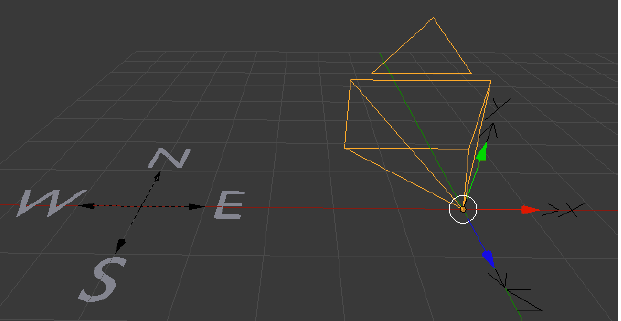
\includegraphics[width=.6\linewidth]{conventions}
\end{figure}
3D world coordinates and their transformations were specified in a \textbf{map} with a center in the origin and the x-axis ranging from west to east, the
z coordinate ranging from north to south and the y-axis orthogonal to the plane.\\
The goal is to find a mapping between a geographical map and the world coordinates in the 3D space. \\

\subsection{View Matrix}
The view matrix assumes that the \textbf{projection plane} (= the screen) is the xy axis.
\begin{itemize}
\item Parallel projection : projection ray is parallel to \textbf{z-axis}
\item Perspective projection : center of projection is the \textbf{origin}
\end{itemize}
Changing the way in which the world is seen (position of object or direction in which we are looking) can be achieved by adding some \textbf{transformations} that are perform \textbf{before} the projections.\\
We can think of the projections matrix as a \textbf{virtual camera} that looks at the screen from the center of projection. It has:
\begin{itemize}
\item \textbf{position} ( initially in origin)
\item \textbf{direction} it is aiming towards (initially along negative z-axis)
\end{itemize}
\begin{figure}[H]
  \centering
  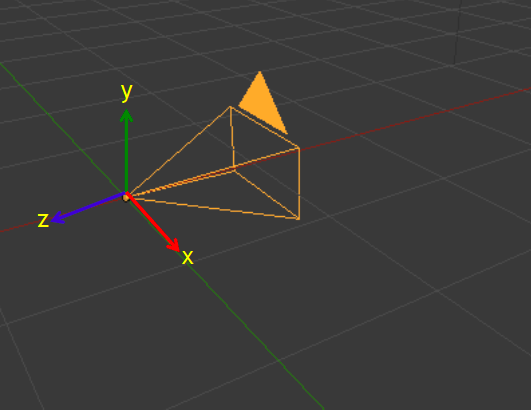
\includegraphics[width=.6\linewidth]{virtualcam}
\end{figure}
The camera can be moved by applying a transformation matrix $M_c$ (\textbf{camera matrix)} that moves the camera object to its position and direction.
Now that the camera is in its new position \textbf{all} objects are moved by applying the \textbf{inverse} matrix $M_c^{-1}$ so that the new projection plane is parallel to the xy-plane and the center of projection is in the origin.\\
The matrix $M_c^{-1}$ is called \textbf{View Matrix} $M_v = M_c^{-1}$.\\
To create the view matrix in a user-friendly way (two most popular):
\begin{itemize}
\item \textbf{look-in direction matrix}
\item \textbf{look-at matrix}
\end{itemize}

\subsubsection{Look-in-direction matrix}
It's the one used in first person games in which you want to see the world in a fixed point and change the direction where you're looking at and the position from which you look the world at.\\
In this kind of model we have (these are just conventions):
\begin{itemize}
\item $(c_x,c_y,c_z) $ position of the center of the camera in world coordinates
\item $\alpha$ horizontal angle = where you look at.
\begin{itemize}
\item $\alpha = \ang{0}  \to$ look north
\item $\alpha = \ang{90} \to$ look west
\item $\alpha = \ang{-90} \to $ look east
\item $\alpha =  +/- \ang{180} \to$ look south
\end{itemize}
\item $\beta $ vertical angle = look up and down
\begin{itemize}
\item $\beta > \ang{0}  \to$ look up
\item $\beta < \ang{0}  \to$ look down
\end{itemize}
\item $\rho$ roll over the viewing angle  = tilting (not often used)
\begin{itemize}
\item $\rho > \ang{0}  \to$ turn counter clockwise
\item $\rho < \ang{0}  \to$ turn clockwise
\end{itemize}
\end{itemize}
\begin{figure}[H]
  \centering
  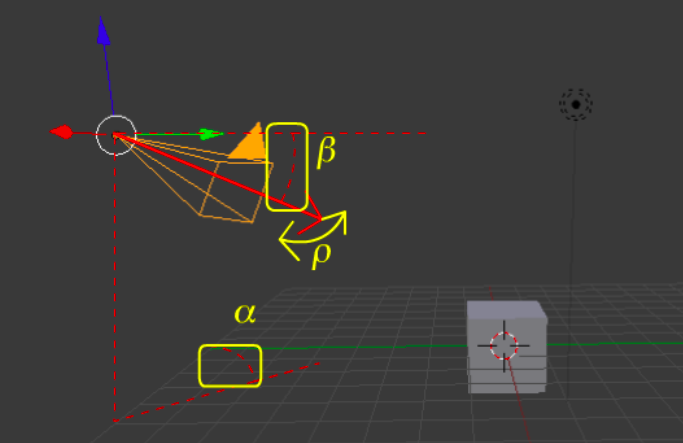
\includegraphics[width=.6\linewidth]{lookindirection}
\end{figure}
The \textbf{View Matrix} is the inverse of this camera matrix so :
$$ M_c = T(c_x,c_y,c_z) \cdot R_y(\alpha) \cdot R_x(\beta) \cdot R_z(\rho)$$
$$ M_v= M_c^{-1} = R_z(-\rho)\cdot R_x(-\beta) \cdot R_y(-\alpha) \cdot T(-c_x,-c_y,-c_z)$$
So to obtain the normalized coordinates of a point A in space seen from a certain point of view :
$$ A'=P_{proj} \cdot M_v \cdot A$$

\subsubsection{Look-at matrix}
This model has :
\begin{itemize}
\item $(c_x,c_y,c_z)$ position of center of the camera
\item $(a_x,a_y,a_z)$ position of the object aimed at
\item $(u_x,u_y,u_z) $ up vector (usually u= (0,1,0) in the y direction)
\end{itemize}
These two points are not enough as they do not decide the \textbf{roll} of the camera. To specify the orientation of the camera the \textbf{up vector} is added.
It is the inverse of gravity and shows which way is up in the world. The camera bottom axis should always be \textbf{perpendicular} to the up vector : this way when you roll the camera is always aligned with the ground.\\
\begin{figure}[H]
  \centering
  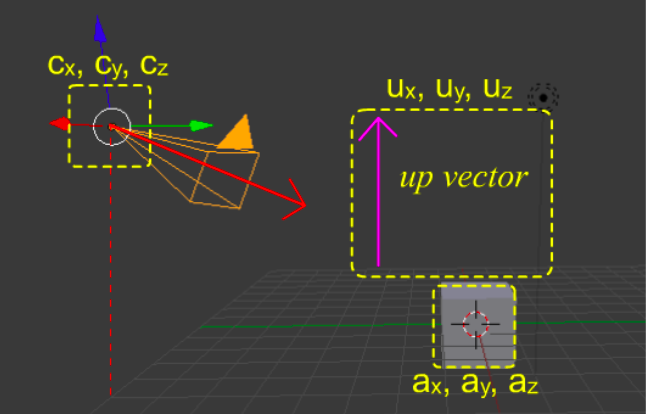
\includegraphics[width=.6\linewidth]{lookat}
\end{figure}
\newpage
The view matrix again is determined starting from the camera matrix.
$$ v_z = \frac{c-a}{|c-a|}$$
$$ v_z = \frac{(c_x-a_x,c_y-a_y,c_z-a_z)}{\sqrt[]{(c_x-a_x)^2+(c_y-a_y)^2+(c_z-a_z)^2}} $$
\begin{figure}[H]
  \centering
  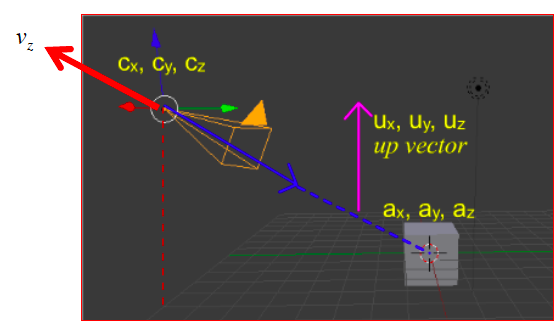
\includegraphics[width=.4\linewidth]{vz}
\end{figure}
The x-axis is perpendicular to both the new z-axis and the up vector 
$$ v_x = \frac{u \times v_z}{|u \times v_z|}$$
$$ u \times v_z = |u_x,u_y,u_z| \times |v_x,v_y,v_z| = |u_yv_z-u_zv_y,u_zv_x-u_xv_z,u_xv_y-u_yv_x|$$
The y-axis is perpendicular to both the new z-axis and the x-axis :
$$ v_y = v_z \times v_x$$
Which leads to 
\[
\boxed{M_c=\begin{array}{c|c}
  v_x \quad v_y \quad v_z& c \\ 
  \hline
  0 \quad 0 \quad 0  & 1
 \end{array} = \begin{array}{c|c}
  R_c & c \\ 
  \hline
  0 & 1
 \end{array}}
\]
Where R is the rotation matrix
So the \textbf{View Matrix} is: 
\[
\boxed{M_v=M_c^{-1}=\begin{array}{c|c}
  R_c^{T} & -(R_c)^T \cdot c \\ 
  \hline
  0  & 1
 \end{array}}
\]
\newpage
\subsection{Local coordinates and World Matrix}
One of the main features of 3D graphics is showing \textbf{moving objects}. Moving is achieved with a \textbf{World Matrix}.\\
Every object is characterized by a set of \textbf{local coordinates}: the positions of the object's points in the space where it was created. When a scene is composed the position of the objects is moved from where it was modelled to where is must be shown . This transformation assigns to the objects new coordinates : the \textbf{global/world coordinates}.\\
\begin{figure}[H]
  \centering
  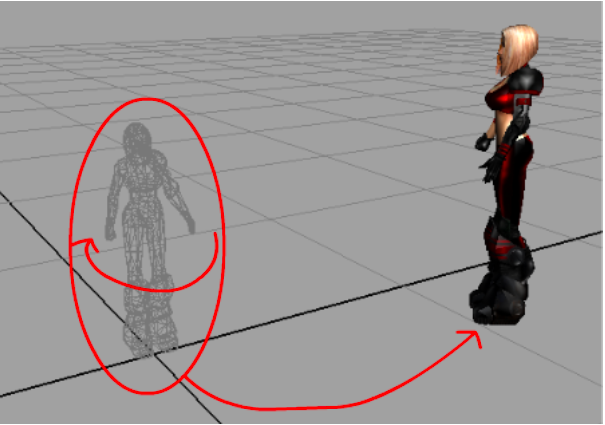
\includegraphics[width=.5\linewidth]{localtoworld}
\end{figure}
The world matrix $M_w$ transforms (translations,rotation,scaling,shear) the local coordinates into the corresponding world coordinates.\\
There are many definitions of transformation order applied to objects with one dominating :
\begin{enumerate}
\item \textbf{Scale/Mirror} the object
\item \textbf{Rotate} the object
\item \textbf{Position} the object
\end{enumerate}

\subsubsection{World Matrix : scaling}
Must be performed first: if the object is scaled or mirrored of $s_x,s_y,s_z$ any rotation must be applied after otherwise it will cause scaling along an arbitrary axis.\\
Scaling makes the objects larger/smaller. If the scaling is proportional is happens equally along all axis. No proportional scaling happens on a specific axis. Applying scaling $s_x,s_y,s_z$ to unitary local coordinates translates into $s_x,s_y,s_z$ global units in the global coordinate system.

\subsubsection{World Matrix : rotating}
Must be performed between scaling and positioning.\\
To define a specific orientation in 3D space a combination of rotations along the 3-axis must be performed. In which order must these rotation be performed?\\
Several ways exist to compute the rotation of the object. A consistent way to specify the parameters required by the user to define orientation in 3D space of an object consists in the \textbf{Euler Angles} :
\begin{itemize}
\item \textbf{ Roll (x-axis)}\\
The roll $ \phi$ identifies the rotation of the object along the facing axis.A \textbf{positive} roll turn an object\textbf{clockwise} in the direction it is facing.
\item \textbf{Pitch (y-axis)}\\
The pitch $\theta$ defines the elevation of the object and corresponds to a rotation around its side axis. A \textbf{positive} pitch turns the head of the object \textbf{facing down}.
\item \textbf{ Yaw (z-axis)}\\
The yaw $\psi$ defines the direction of the object and corresponds to a rotation along the vertical axis. $\psi = \ang{0} \to$ East
\end{itemize}
Euler angles are defined for a z-up coordinates system.
\begin{figure}[H]
  \centering
  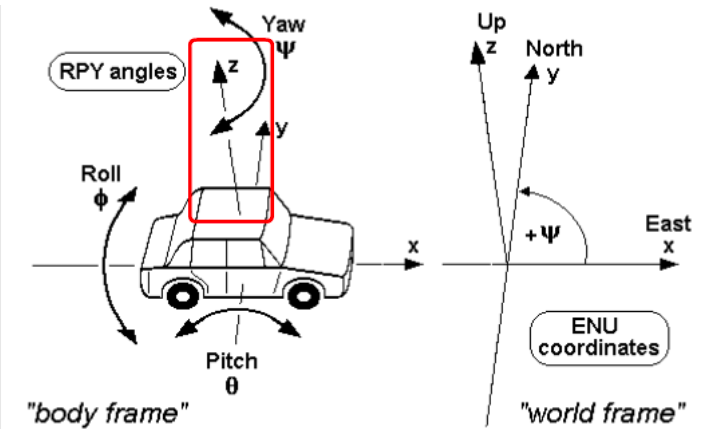
\includegraphics[width=.5\linewidth]{zup}
\end{figure}
Object are modelled so that they face the positive x-axis, the side aligned with the y-axis and vertically along the z-axis.\\ 
With the above conventions transformations are performed in the alphabetical order:
\begin{enumerate}
\item x-axis $\to$ Roll
\item y-axis $\to$ Pitch
\item z-axis $\to$ Yaw
\end{enumerate}
If the axis conventions are different the order must always be Roll-Pitch-Yaw
\begin{figure}[H]
  \centering
  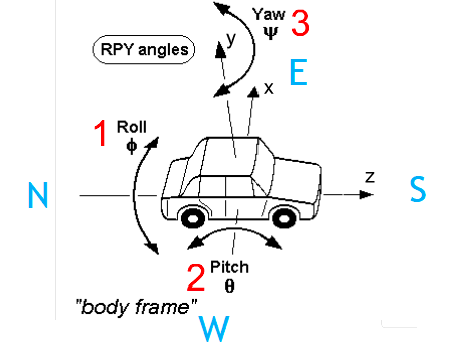
\includegraphics[width=.5\linewidth]{diffconv}
\end{figure}
For example in the 'Look-in-direction' camera model a y-up Euler angle orientation system was used. The camera is however oriented in the negative z-axis. For this reason the Roll $\phi$ and Pitch $\theta$ work in the opposite way as $\rho$ and $\beta$ and direction $ \alpha = 0$ corresponds to the camera looking North instead of South.Rotations are still performed in the same order.

\subsubsection{World Matrix : positioning}
Must be performed last otherwise the coordinates would be changed during the other transformation.\\
When positioning the object the user wants to specify the coordinates where it should be placed in the 3D place.These coordinates should be independent of the size and orientation of the object.\\
Positioning at $p=(p_x,p_y,p_z)$ is performed by applying a \textbf{transformation} $T(p_x,p_y,p_z)$. So $(p_x,p_y,p_z)$ are the coordinates of the origin of the object after the transformations ( initially is the origin in local coordinates was $(0,0,0)$ )

\subsubsection{Final World Matrix}
With this y-up convention (object facing the positive z-direction , x is the side direction )an object in space can be positioned in a 3D space using 9 parameters:
\begin{itemize}
\item position $p_x,p_y,p_z$
\item rotation $\phi, \psi,\theta,$
\item scaling $s_x,s_y,s_z$
\end{itemize}
\begin{figure}[H]
  \centering
  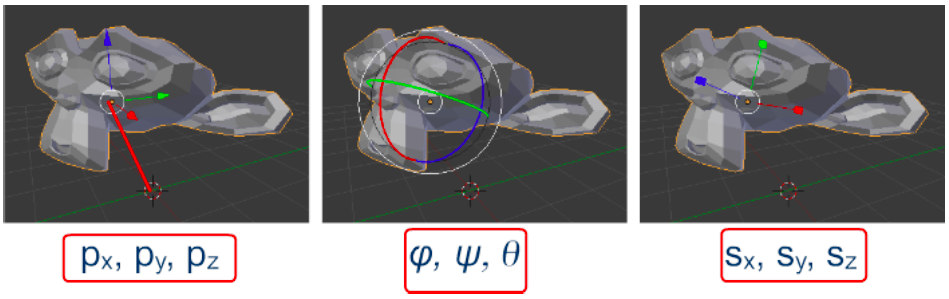
\includegraphics[width=.5\linewidth]{9params}
\end{figure}
The final world matrix is :
\[
\boxed{M_w = T(p_x,p_y,p_z)\cdot R_y(\psi) \cdot R_x(\theta) \cdot R_z(\phi) \cdot S(s_x,s_y,s_z)}
\]

\subsection{Gimbal Lock}
A rotation defined by the Euler Angles is perfect for \textbf{planar} movements ( good for driving games or FPS).Euler Angles are a problem for applications such as flight simulators as they suffer from a problem known as \textbf{gimbal lock}.
A \textbf{gimbal} is a ring that can spin around its diameter.
\begin{figure}[H]
  \centering
  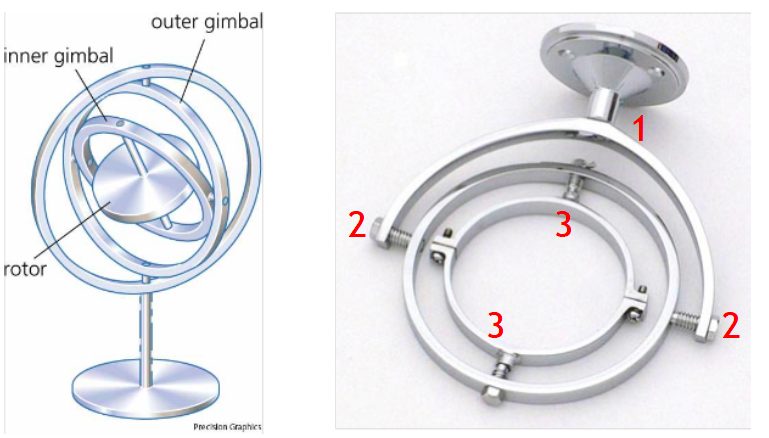
\includegraphics[width=.4\linewidth]{gimbal}
\end{figure}
A physical system that allows freely orienting an object in the space has \textbf{at least three} gimbals connected to each other (one for each rotation roll-pitch-yaw).
The problem is that the rotations are connected : each ring corresponds to a rotation along x,y,z -axis. Consider an order of y-x-z as in figure below
\begin{figure}[H]
  \centering
  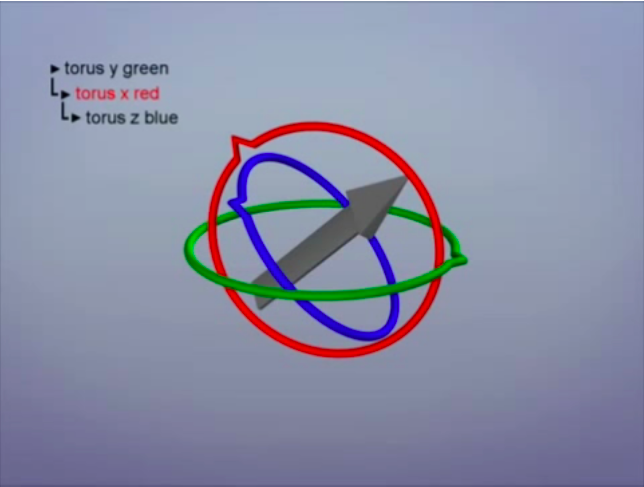
\includegraphics[width=.5\linewidth]{gimbalordering}
\end{figure}
Moving the yaw (green outermost ring) a movement of the other two rings can be observed. Moving the the pitch (red middle ring) the roll (blue inner ring) moves too.\\
If the pitch (x-axis) rotates 90 degrees , the z and y axis are \textbf{aligned}
\begin{figure}[H]
  \centering
  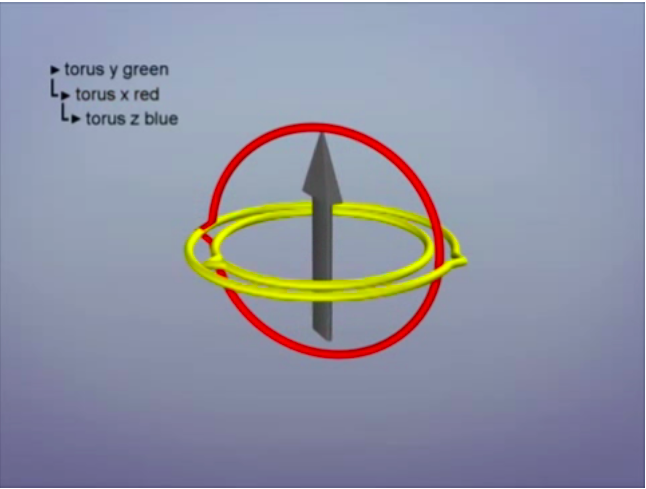
\includegraphics[width=.4\linewidth]{gimbalaligned}
\end{figure}
So we \textbf{loose} a degree of freedom. When a \textbf{gimbal lock} occurs some movements are no longer performable: such movements must be performed by doing complex \textbf{combinations} of these movements. In our case a common solution used to express the rotation of an object is to use a mathematical device called \textbf{quaternion} instead of Euler Angles.